\chapter{Materiais e Métodos}
\label{metodologia_ref}
\phantom{0}
  
Este capítulo descreve os procedimentos utilizados para diagnóstico dos padrões de interferência da camada lipídica do filme lacrimal, a partir de imagens capturadas com o Interferômetro Doane e Tearscope Plus. Primeiramente são apresentadas as bases de imagens classificadas como um problema multiclasse, nas quais será aplicado o método proposto. Em seguida, é descrita a sequência de etapas realizadas para alcançar o objetivo proposto no método.

\section{Base de Imagens Capturadas com o Interferômetro Doane}
\label{sec:metodoBaseInterferometrica}

A base de imagens VOPTICAL\_GCU \cite{voptical_gcuvarpa2013} contém imagens interferométricas do filme lacrimal, adquiridas de pacientes com a Síndrome do Olho Seco com faixa etária entre 16 e 55 anos. Todas as imagens foram disponibilizadas por dois optometristas do Departamento de Ciências da Vida, da Universidade Caledoniana de Glasgow (Glasgow, Reino Unido).

Nesta base de imagens, a aquisição foi feita usando o Interferômetro Doane \cite{doane1989instrument} e uma câmera digital CMEX-1301. Como o filme lipídico lacrimal não é estático entre os flashes, um vídeo foi gravado e a melhor imagem para processamento foi selecionada. As imagens têm uma resolução de 1280x1024 \textit{pixels} no espaço de cor RGB. A base contém 106 imagens das cinco categorias consideradas: 11 franjas fortes, 25 coalescentes de franjas fortes, 30 franjas finas, 26 coalescentes de franjas finas e 14 detritos. A~\autoref{fig:baseInterferometrica} ilustra exemplos das cinco categorias.

\begin{figure}[ht!]
    \centering
    \caption{Categorias da camada lipídica das imagens da base VOPTICAL\_GCU: (a) franjas fortes; (b) coalescentes de franjas fortes; (c) franjas finas; (d) coalescentes de franjas finas; (e) detritos.}
    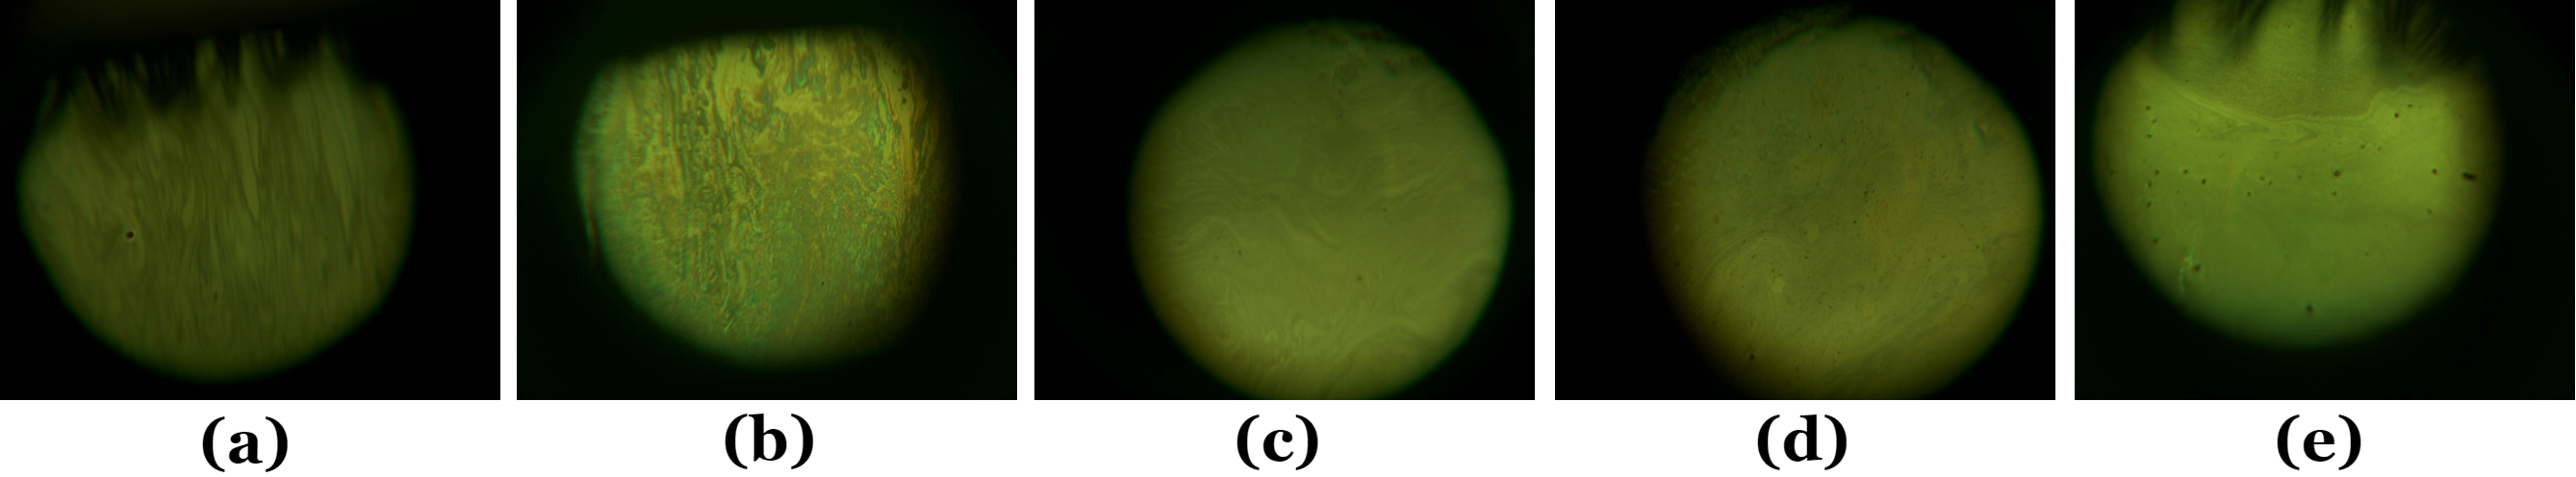
\includegraphics[width=15.8cm]{figs/BaseVOPTICAL.png}
    \legend{Fonte: \cite{voptical_gcuvarpa2013}.}
    \label{fig:baseInterferometrica}
\end{figure}

No estudo realizado por \citeonline{remeseiro2015automatic}, as categorias dos padrões de interferência das imagens foram definidas por optometristas da seguinte forma: (a) franjas óbvias de cor com uma aparência de se espalhar pela córnea; (b) franjas de cores óbvias, mas aglomerando-se em ilhas de cor; (c) franjas cinza com uma aparência de propagação através da córnea; (d) franjas cinza, mas aglomerando-se em ilhas de cinza; e (e) distúrbios óbvios no filme lacrimal, provavelmente de origem variada.

\section{Bases de Imagens Capturadas com o Tearscope Plus}
\label{sec:metodoBaseTearscope}

Os conjuntos de bases VOPTICAL\_I1, VOPTICAL\_I1-v2 e  VOPTICAL\_Is contêm imagens do filme lacrimal pré-ocular adquiridas do mesmo grupo de pacientes com idades entre 19 e 33 anos. A aquisição das imagens foi realizada com o Tearscope Plus (Keeler Ltd., Reino Unido)  \cite{guillon1997tearscope} acoplado a uma lâmpada de fenda Topcon SL-D4 e uma câmera digital Topcon DV-3. Um vídeo foi gravado e a melhor imagem foi selecionada. Todas as imagens têm uma resolução de 1024x768 \textit{pixels} e estão no espaço de cor RGB. Estes conjuntos de imagens foram adquiridos e anotados por optometristas do Serviço de Optometria da Universidade de Santiago de Compostela (Espanha).

O Tearscope Plus permite aos médicos avaliar rapidamente a espessura da camada lipídica. \citeonline{guillon1998non} definiu uma escala de classificação composta de cinco categorias, que em espessura crescente são: malha aberta, malha fechada, onda, amorfa e franja de cor.

%O tacoplado a uma lâmpada de fenda Topcon SL-D4 e uma câmera digital Topcon DV-3. A ampliação do biomicroscópio foi ajustada para 200X e as imagens armazenadas com uma resolução de 1024 768 pixels. Como o lípide lacrimal lm não é estático entre os flashes, um vídeo foi gravado e analisado para selecionar as imagens a serem processadas: uma imagem foi selecionada somente quando o lípide do lípido lacrimal foi completamente expandido após o piscar do olho.

%O Tearscope Plus, projetado por Guillon [1], é o instrumento de escolha para a avaliação da espessura da camada lipídica em ambientes clínicos. Guillon também propôs cinco principais categorias de lipídios

%Guillon também propôs cinco graus principais de padrões de interferência da espessura da camada lipídica para observações feitas usando o Tearscope Plus: malha aberta (10–20 nm), malha fechada (20–50 nm), onda (50–70 nm), amorfa (80–90 nm) e cor de franja (90–180 nm). Outros padrões associados à patologia ocular frequentemente aparecem como franjas anormais de cor, referidas como padrões globulares (> 180 nm).

%Observe que a espessura da camada lipídica está associada aos olho SF, pois uma camada lipídica mais fina acelera a evaporação da água.
%Os nomes dos arquivos das imagens indicam o padrão de interferência predominante: CO é franja de cor, AM é amorfo, FL é onda, MA é malha aberta e MC é malha fechada.

\subsection{Bases VOPTICAL\_I1 e VOPTICAL\_Is}
\label{subsec:basesI1eIs}

Embora os padrões de interferência sejam independentes da iluminação, existe uma faixa ótima de iluminações usadas pelos optometristas para obter as imagens. Imagens com iluminações fora deste intervalo são consideradas imagens ruidosas \cite{remeseiro2014methodology}. Dessa maneira, dois conjuntos de imagens foram gerenciados. A primeira base contém 105 imagens do conjunto VOPTICAL\_I1 \cite{voptical_gcuvarpa_i1}, todas nas mesmas condições de iluminação, distribuídas em 29 malhas abertas, 29 malhas fechadas, 25 de ondas e 22 de franja de cor.

A segunda base contém 406 imagens do conjunto de imagens VOPTICAL\_Is \cite{voptical_gcuvarpa_is}, em diferentes condições de iluminação. Esta base possui 159 malhas abertas, 117 malhas fechadas, 90 ondas e 40 franja de cor. Não contém imagens dentro da categoria amorfa porque é um padrão muito incomum \cite{garcia2013new}, e por esta razão a última categoria não foi considerada nessas duas bases.

A~\autoref{fig:2basesTeascope} mostra exemplos de imagens das categorias da camada lipídica em ambas as bases. As imagens superiores compõem a base VOPTICAL\_I1, e as inferiores a base VOPTICAL\_Is. As imagens da base VOPTICAL\_Is possuem uma iluminação muito alta, produzindo uma imagem onde o padrão de interferência é dificilmente apreciado.

\begin{figure}[ht!]
    \centering
    \caption{Categorias da camada lipídica. Imagens superiores são da base VOPTICAL\_I1 e inferiores VOPTICAL\_Is: (a) malhas abertas; (b) malhas fechadas; (c) ondas; (d) franja de cor.}
    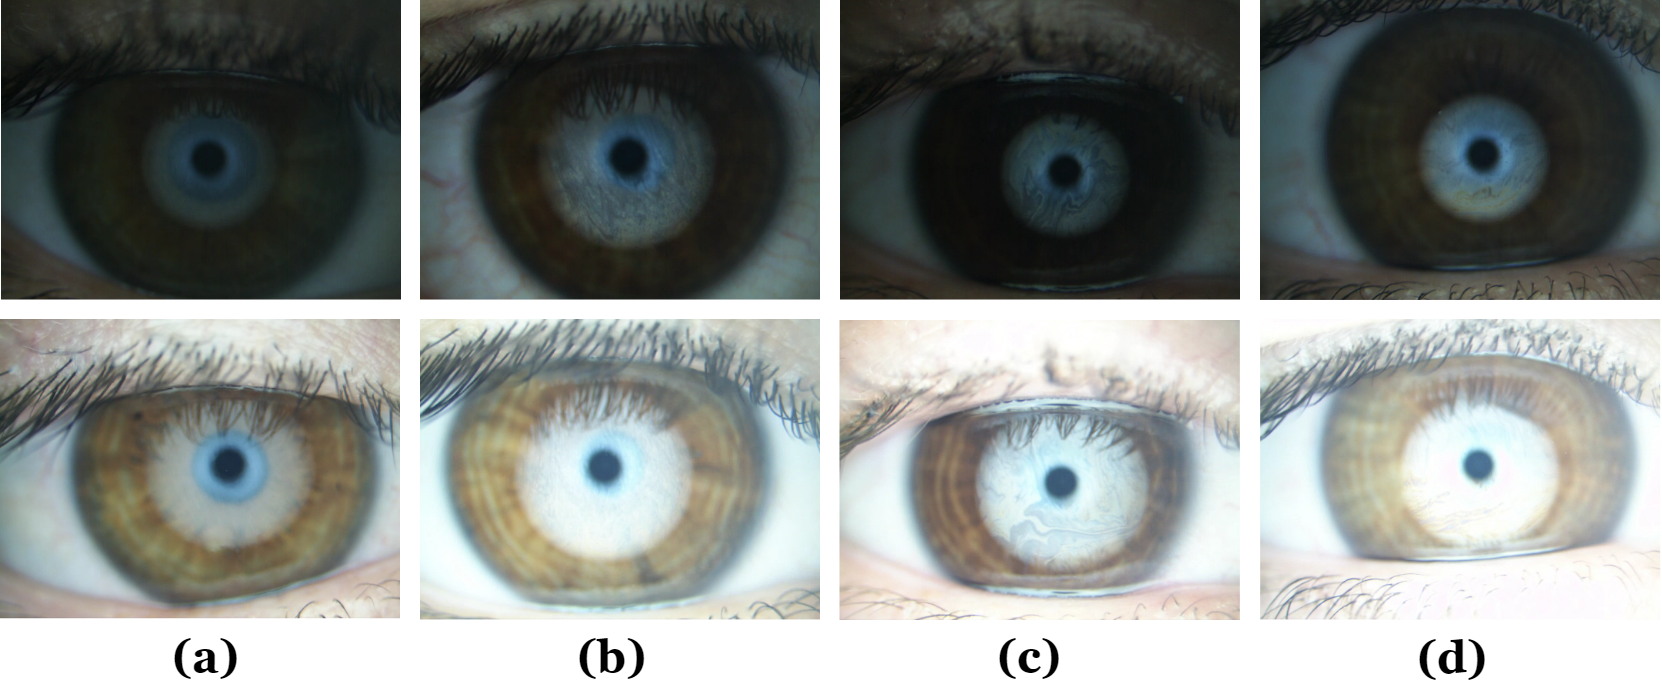
\includegraphics[width=15.4cm]{figs/DuasBases1.png}
    \legend{Fonte: \cite{voptical_gcuvarpa_i1, voptical_gcuvarpa_is}.}
    \label{fig:2basesTeascope}
\end{figure}

\subsection{Base VOPTICAL\_I1-v2}

O conjunto de imagens VOPTICAL\_I1-v2 \cite{voptical_gcuvarpa_i1-v2} é a versão atualizada do conjunto de imagens VOPTICAL\_I1 e inclui a categoria amorfa. A base contém 128 imagens do filme lacrimal adquiridas de pacientes com olhos escuros. O conjunto de imagens têm 29 malhas abertas, 29 malhas fechadas, 25 ondas, 23 amorfas e 22 franja de cor. A~\autoref{fig:basesVersao2Teascope} demonstra exemplos das cinco categorias da camada lipídica.

\begin{figure}[ht!]
    \centering
    \caption{Categorias da camada lipídica das imagens da base VOPTICAL\_I1-v2: (a) malhas abertas; (b) malhas fechadas; (c) ondas; (d) amorfas; (e) franja de cor.}
    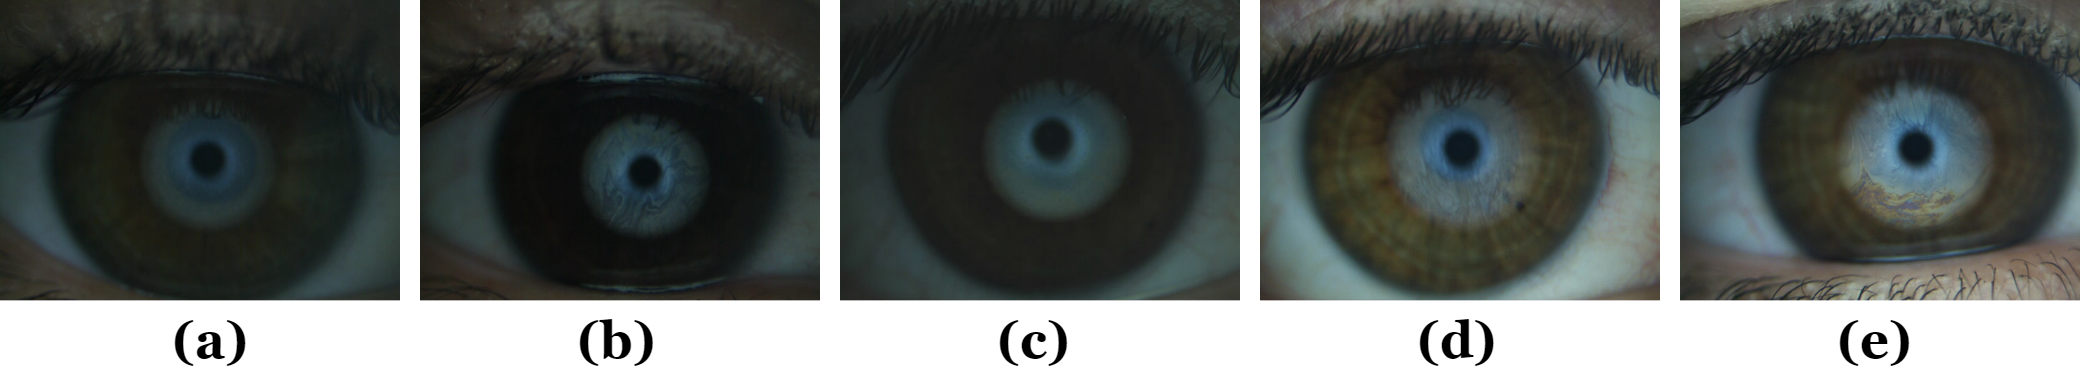
\includegraphics[width=15.8cm]{figs/BaseVersao2.png}
    \legend{Fonte: \cite{voptical_gcuvarpa_i1-v2}.}
    \label{fig:basesVersao2Teascope}
\end{figure}

\section{Método Proposto}
\label{sec:metodoProposto}

%O método proposto consiste em quatro etapas: segmentação, extração de características, seleção de características e reconhecimento de padrões. A~\autoref{fig:metodoProposto} ilustra a sequência que essas etapas são executadas. Na primeira etapa é realizado a segmentação das quatro bases de imagens, uma capturada com o Interferômetro Doane e três com o Teascope Plus. Na segunda etapa é realizado a extração de características com os descritores de textura baseados em índices de diversidade filogenéticos, que são aplicados somente nas imagens capturadas com o Interferômetro Doane, e a função K de \textit{Ripley} nas imagens capturadas com o Teascope Plus.

%As características mais discriminantes dos vetores de características extraídos são selecionados na terceira etapa e, submetidos como entrada para o processo de classificação supervisionada (quarta etapa) usando os classificadores Random Forest, SVM, Naive Bayes e Bayes Net. Finalmente, os resultados são validados utilizando métricas de desempenho e comparados com os resultados encontrados na literatura.

%O método proposto consiste em quatro etapas: segmentação, extração de características, seleção de características e reconhecimento de padrões. Foram realizados testes separadamente para cada base de imagens, a Seção~\ref{sec:resultadosDisc} apresentará os resultados obtidos em cada um dos experimentos. Para cada tipo de base de imagens, os fluxos apresentam sequências diferentes em algumas etapas. A~\autoref{fig:metodoProposto} ilustra a sequência que as etapas são executadas.

%O método proposto consiste em quatro etapas: segmentação, extração de características, seleção de características e reconhecimento de padrões. Para cada tipo de base de imagens, os fluxos apresentam sequências diferentes em algumas etapas e, consequentemente, serão apresentados os resultados para os diferentes tipos de bases de imagens. A~\autoref{fig:metodoProposto} ilustra a sequência que as etapas são executadas.

O método proposto consiste em quatro etapas: segmentação, extração de características, seleção de características e reconhecimento de padrões. A~\autoref{fig:metodoProposto} ilustra a sequência que as etapas são executadas. Para cada tipo de base de imagens, os fluxos apresentam sequências diferentes em algumas etapas, e são realizados testes separadamente para cada base de imagens, o Capítulo~\ref{sec:resultadosDisc} apresentará os resultados obtidos em cada um dos experimentos.

Na primeira etapa realiza-se a segmentação da região de interesse nas imagens das quatro bases, uma capturada com o Interferômetro Doane e três com o Tearscope Plus. Na segunda etapa é realizado a extração de características com os descritores de textura baseados em índices de diversidade filogenética, que são aplicados nas imagens da base capturada com o Interferômetro Doane; e a função K de \textit{Ripley} nas imagens das bases capturadas com o Tearscope Plus e Interferômetro Doane.

As características mais discriminantes dos vetores de características extraídos são selecionadas na terceira etapa para todas as bases de imagens, posteriormente, são submetidas como entrada para o processo de classificação supervisionada (quarta etapa) usando os classificadores \textit{Random Forest}, \textit{Support Vector Machine}, \textit{Naive Bayes} e \textit{Bayes Net}. Finalmente, os resultados obtidos são validados utilizando métricas de desempenho e comparados com os resultados encontrados na literatura.

%As características mais discriminantes dos vetores de características extraídos são selecionados na terceira etapa e, submetidos como entrada para o processo de classificação supervisionada (quarta etapa) usando os classificadores Random Forest, SVM, Naive Bayes e Bayes Net. Finalmente, os resultados são validados utilizando métricas de desempenho e comparados com os resultados encontrados na literatura.

\begin{comment}
O método proposto consiste em quatro etapas: segmentação, extração de características, seleção de características e reconhecimento de padrões. A~\autoref{fig:metodoProposto} ilustra a sequência que as etapas são executadas para o fluxo (1) que utiliza base de imagem capturada com o Interferômetro Doane; e o fluxo (2) bases de imagens capturadas com o Tearscope Plus. Pode ser observado que os fluxos (1) e (2) apresentam sequências diferentes em algumas etapas e, consequentemente, serão apresentados os resultados para os diferentes fluxos.

Em geral, a primeira etapa é realizado a segmentação da região de interesse nas quatro bases de imagens, em que uma base é capturada com o Interferômetro Doane e três com o Tearscope Plus. Na segunda etapa é realizado a extração de características com os descritores de textura baseados em índices de diversidade filogenética no fluxo (1), e a função K de \textit{Ripley} no fluxo (1) e (2).

As características mais discriminantes dos vetores de características extraídos são selecionados na terceira etapa em ambos os fluxos e, submetidos como entrada para o processo de classificação supervisionada (quarta etapa) usando os classificadores \textit{Random Forest}, \textit{Support Vector Machine}, \textit{Naive Bayes} e \textit{Bayes Net}. Finalmente, os resultados dos fluxos são validados utilizando métricas de desempenho e comparados com os resultados encontrados na literatura.
\end{comment}

\begin{figure}[ht!]
    \centering
    \caption{Etapas do método proposto.}
    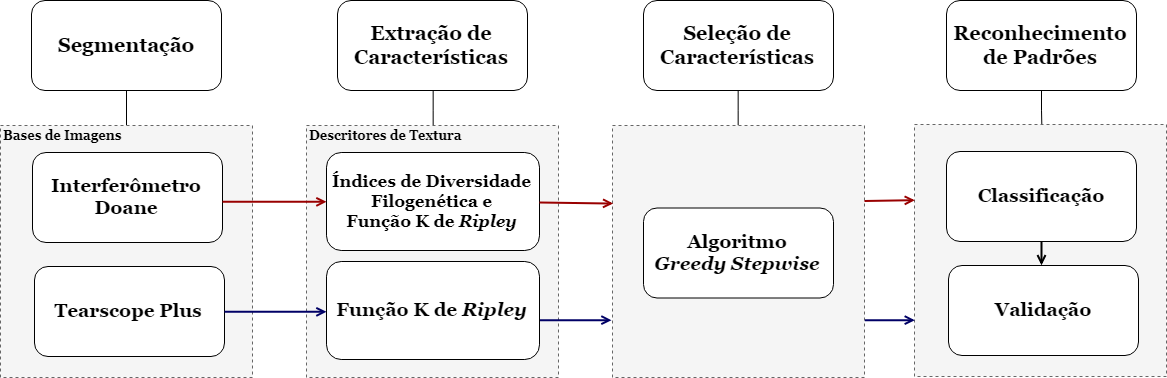
\includegraphics[width=15.8cm]{figs/metodoDissertacao2.png}
    \legend{Fonte: Elaborado pela autora.}
    \label{fig:metodoProposto}
\end{figure}

\subsection{Segmentação}
\label{sec:metodoSegmentacao}

%A segmentação consiste na separação dos objetos de interesse de informações irrelevantes presentes em imagens digitalizadas. As Seções seguintes apresentam duas segmentações diferentes referentes as quatro bases de imagens, divididas em dois grupos de tipos de imagens, utilizando o Interferômetro Doane (base VOPTICAL\_GCU) e o Tearscope Plus (base VOPTICAL\_I1, VOPTICAL\_I1-v2 e VOPTICAL\_LS).

A segmentação consiste na separação dos objetos de interesse, de informações irrelevantes presentes em imagens digitalizadas. As seções seguintes apresentam duas segmentações diferentes referentes aos tipos de imagens capturadas com o Interferômetro Doane (base VOPTICAL\_GCU) e as capturadas com Tearscope Plus (base VOPTICAL\_I1, VOPTICAL\_I1-v2 e VOPTICAL\_Is).


%Na segmentação manual todo o processo de separação de um objeto de interesse é conduzido por um especialista humano, o que torna o procedimento exaustivo e custoso. Portanto, faz-se necessário um sistema para segmentação automática das regiões de interesse, visando tornar o trabalho ágil e menos custoso. Nesta dissertação foram utilizadas quatro bases de imagens, e realizadas duas segmentação diferentes para os tipos de imagem que compõem as bases. A seguir são detalhados tais procedimentos.

\subsubsection{Segmentação das ROIs de Imagens Capturadas pelo Interferômetro Doane}
\label{sec:metodoSegInterferometroDoane}

As imagens de entrada adquiridas com o Interferômetro Doane, incluem áreas irrelevantes presentes nas áreas externas, como ilustrado na~\autoref{fig:ExtracaoROI} (a). Assim, a região mais relevante para segmentação encontra-se na parte central da área amarelada ou esverdeada da imagem, formada pela superfície anterior do filme lacrimal que cobre a córnea. Portanto, foi realizado um passo destinado à extração da ROI, conforme proposto em \cite{remeseiro2015automatic}.

\begin{figure}[ht!]
    \centering
    \caption{Etapas da segmentação da ROI de imagens capturadas com Interferômetro Doane.}
    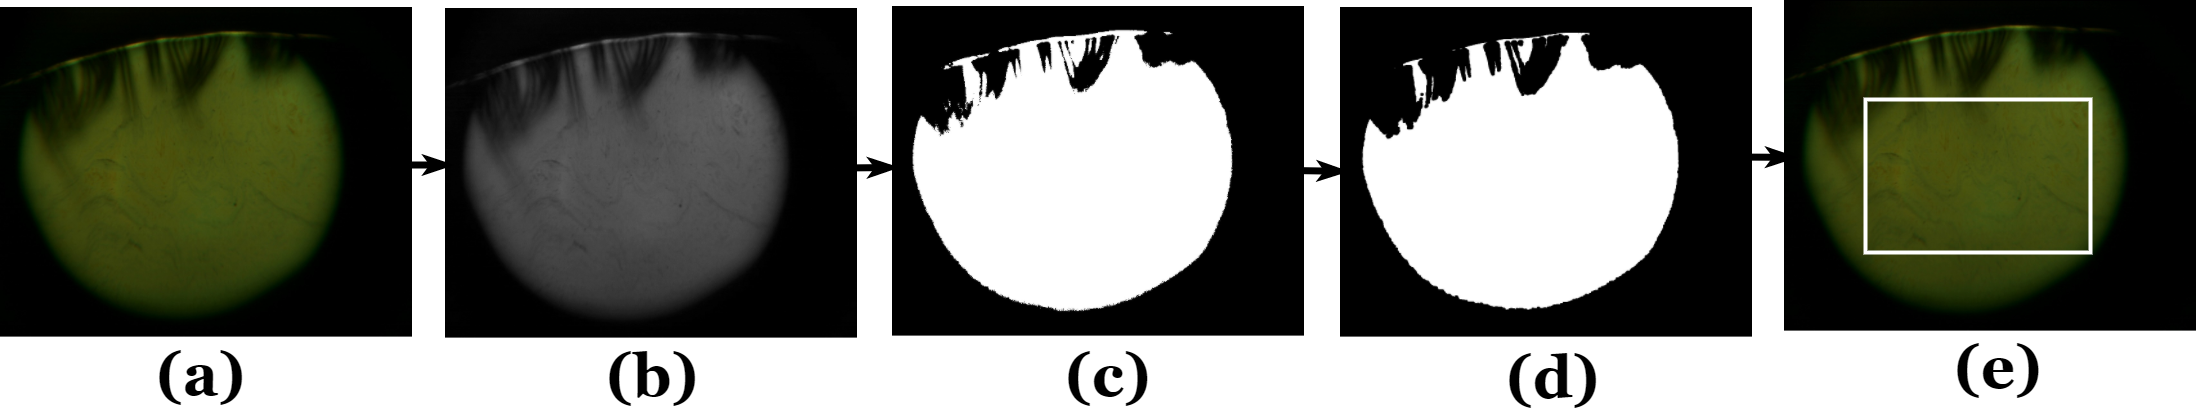
\includegraphics[width=15.8cm]{figs/ExtracaoROI.png}
    \legend{Fonte: Elaborado pela autora.}
    \label{fig:ExtracaoROI}
\end{figure}

A região relevante da imagem é caracterizada por tonalidades esverdeadas ou amareladas, assim apenas o canal verde (G) da imagem de entrada em RGB é considerado (\autoref{fig:ExtracaoROI} (b)). Na imagem do canal G é usado o princípio de limiar, que consiste em separar os \textit{pixels} da imagem em duas classes (fundo e objeto). O objetivo é encontrar os \textit{pixels} cujo nível de cinza é menor que um limite (\autoref{fig:ExtracaoROI} (c)). O cálculo desse limite é apresentado na~\autoref{equacao:equacaoLimiar}.

\begin{equation}
\label{equacao:equacaoLimiar}
limiar = media - p  \times \sigma,
\end{equation}onde $media$ constitui o valor médio dos níveis de cinza da imagem, $\sigma$ é o desvio padrão e $p$ é um fator de peso empiricamente determinado ($p$ = 0,1). Depois que a ROI preliminar é identificada, sua parte central deve ser localizada. Devido algumas imagens incluírem outras regiões irrelevantes, como cílios, o operador morfológico de erosão \cite{gonzalez2008digital}, usando uma elipse como elemento estruturante é aplicado (\autoref{fig:ExtracaoROI} (d)). Em seguida, um retângulo dentro da região identificada acima é mapeado e reduzido até que nenhuma área do fundo permaneça (\autoref{fig:ExtracaoROI} (e)). Observa-se que o tamanho das imagens de entrada é 1280 x 1024 \textit{pixels}, e o tamanho final da ROI é, em média, 547 x 578 \textit{pixels}.

%Especialistas geralmente se concentram na parte inferior da íris, porque esta é a área onde a lágrima pode ser percebida com o melhor contraste.

\subsubsection{Segmentação das ROIs de Imagens Capturadas pelo Tearscope Plus}
\label{sec:metodoSegTearscopePlus}

As imagens de entrada obtidas com o Tearscope Plus, incluem várias áreas do olho que não contêm informações relevantes para a classificação, conforme ilustrado na~\autoref{fig:ExtracaoROI2} (a). O procedimento de aquisição garante que há uma área central na imagem mais iluminada do que o ambiente ao redor, na qual o filme lacrimal pode ser observado. Consequentemente, optometristas que analisam visualmente essas imagens concentram sua atenção nessa parte da íris, ou seja, na área mais clara entre a pupila e o limite da íris. Portanto, este fato força uma etapa destinada a extração da ROI.

%O procedimento de aquisição garante que esta região corresponda à área mais iluminada da imagem. Para isso, a imagem de entrada é transformada no espaço de cores Lab e somente o componente L é considerado nesta etapa. Além disso, um conjunto de modelos em forma de anel que definem diferentes formas de ROI é usado. Em seguida, a correlação cruzada normalizada entre o componente L e o conjunto de modelos é calculada. Finalmente, a região com o valor máximo de correlação cruzada é selecionada [ver Figura 3 (b)] e a ROI da imagem de entrada é obtida através de um processo completamente automático.

\begin{figure}[ht!]
    \centering
    \caption{Etapas da segmentação da ROI de imagens capturadas com Tearscope Plus.}
    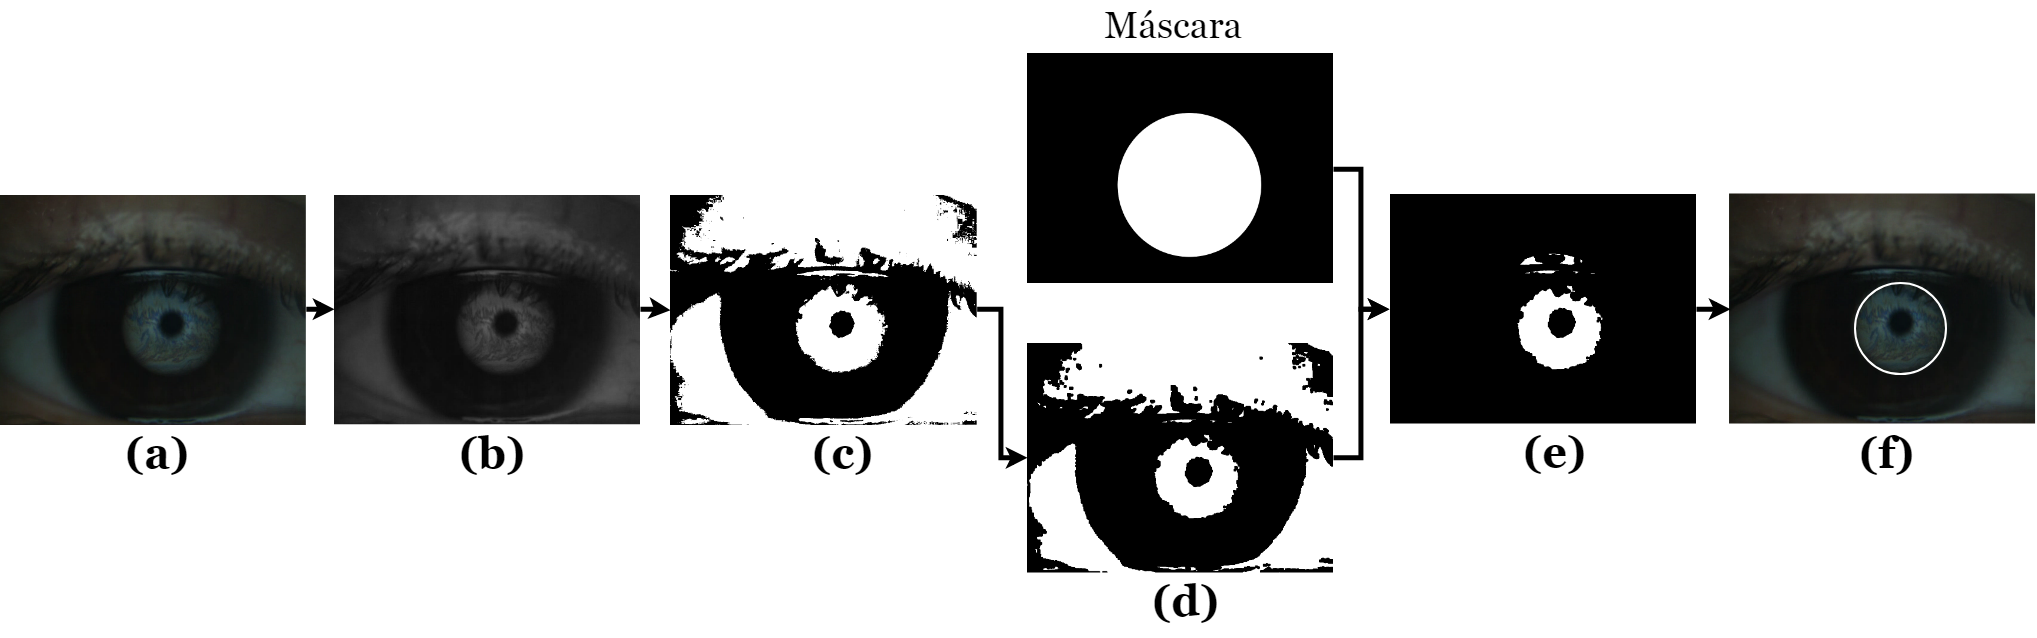
\includegraphics[width=15.8cm]{figs/ExtracaoROI3.png}
    \label{fig:ExtracaoROI2}
    \legend{Fonte: Elaborado pela autora.}
\end{figure}

O filme lacrimal pode ser percebido com o maior contraste no canal verde da imagem de entrada, assim como nas imagens interferométricas. Portanto, as etapas apresentadas na \autoref{fig:ExtracaoROI2} (b), (c) e (d) seguem os mesmos procedimentos encontrados nas etapas da~\autoref{fig:ExtracaoROI} (b), (c) e (d) detalhadas na Subseção~\ref{sec:metodoSegInterferometroDoane}. Em seguida, foi observado que a região de interesse encontra-se sempre um pouco abaixo do centro das imagens. Assim, uma máscara fixa foi utilizada nesta etapa, extraindo apenas as informações que coincidem com a região marcada pela máscara fixa (\autoref{fig:ExtracaoROI2} (e)). Uma vez identificada esta ROI preliminar, pode ser observado que algumas imagens ainda incluem outras regiões que não contêm informações relevantes para a extração de características. Para eliminar essas regiões foram localizadas circunferências no objeto de interesse. Por fim, foi retornado a circunferência que contém maior área, representando a região de interesse para extração de características (\autoref{fig:ExtracaoROI2} (f)).

\subsection{Extração de Características}
\label{sec:metodoExtracao}

Após a extração da ROI, inicializa-se a etapa de caracterização. Esta etapa visa obter medidas descritivas da camada lipídica do filme lacrimal, que formarão os vetores de características a serem utilizados nas etapas de seleção e classificação. O procedimento de extração de características adotado neste trabalho é distribuído em análises de texturas baseadas em geoestatística (Subseção~\ref{sec:kripley}) e índices de diversidade filogenética (Subseção~\ref{sec:indicesDiversidade}). %\cite{doi:10.2989/16085910409503825}

Nas bases de imagens capturadas com o Interferômetro Doane são aplicados os descritores baseados em índices de diversidade filogenética e a função K de \textit{Ripley}. E nas bases capturadas com o Tearscope Plus são aplicadas a função K de \textit{Ripley}. A seguir, são detalhadas as adaptações utilizadas para a extração de características com essas técnicas.

\subsubsection{Extração de Características usando a Função K de \textit{Ripley}}
\label{sec:metodoRipley}

Os índices geostatísticos descrevem a textura em termos de medidas de autocorrelação espacial. A autocorrelação espacial é uma medida de similaridade entre pontos em uma certa distância \cite{clark1979practical}. Especificamente, no contexto deste descritor, é utilizada a representação da ROI em LBP padrão com tamanho de janela $3x3$, onde um ponto analisado em geostatística corresponderá ao padrão binário local na ROI, aplicado sobre os espaços de cores baseado em cores oponentes, L*a*b*, RGB e YCbCr \cite{plataniotis2013color}.

Posteriormente, são aplicadas as abordagens em círculos e anéis apresentadas sobre a função K de \textit{Ripley} (Subseção~\ref{sec:kripley}). O procedimento adotado é semelhante para as duas abordagens. Para diferentes valores de raios $r$, a partir da escolha de um centro $i$, são analisadas as ocorrências de LBPs de um mesmo valor $j$. Foram utilizados 6 raios, parâmetro empiricamente testado, onde valores menores normalmente reduzem o desempenho e valores maiores aumentam a complexidade e não incluem características relevantes. Vale observar que a escolha da quantidade de raios é um critério dependente da abordagem adotada e pode variar entre métodos ou estudos diferentes.

Para determinar os 6 raios é necessário calcular o raio máximo que pode ser alcançado a partir do seu centro, ou seja, a distância entre o centro da ROI até o \textit{pixel} mais distante pertencente à mesma (cálculos apresentados na Seção~\ref{sec:kripley}). A quantidade de raios provê uma divisão das ROIs em círculos ou anéis de tamanhos que crescem gradativamente em variação relativamente pequena de raio, mas não unitária. %Cada raio é definido através da equação:

\begin{comment}
\begin{equation}
\label{equacao:raioRipley}
R_{i} = \frac{R_{Max}}{6}*i \ \ \ \ \ \ \ para \ \ \ i = 1,2,3,4,5,6
\end{equation}
\end{comment}

Além da utilização dos raios, pretende-se encontrar características existentes em agrupamentos de um mesmo padrão, com o objetivo de representar a maior quantidade possível de informações sobre as camadas lipídicas. Para atingir este objetivo, cada ROI foi quantizada sucessivamente de 256 níveis, para 128, 64, 32, 16 e 8, que corresponde a 6 quantizações diferentes para cada um dos 6 raios de amostragem. Além disso, vale ressaltar que foram realizados experimentos exaustivos de quantização e foram apresentados apenas os melhores resultados.

Posteriormente, o LBP foi aplicado sobre o resultado de cada uma das quantizações. Finalmente, cada raio de amostragem gera uma observação sobre cada um dos 3 canais de cada espaço de cores. Dessa forma, são extraídas 3024 características (6 raios x (256 + 128 + 64 + 32 + 16 + 8 quantizações)) para cada canal de cada espaço de cor, totalizando 9072 características.

\subsubsection{Extração de Características usando Índices de Diversidade Filogenética}
\label{sec:metodoIndicesD}

Para descrição da textura, foram utilizados todos os índices de diversidade filogenética apresentados na Seção~\ref{sec:indicesDiversidade}. Esse descritor de textura foi utilizado somente na base de imagens capturadas com os Interferômetro Doane (Subseção~\ref{sec:metodoBaseInterferometrica}) e aplicado sobre o espaço de cor em nível de cinza.

O processo de extração de características usando os índices de diversidade filogenética é semelhante em todos os grupos dos índices filogenéticos. Esses índices são utilizados para analisar a distribuição de espécies em uma região de análise, usados em conjunto com as árvores filogenéticas. Para montar e organizar
a árvore, é necessário saber quais espécies estão presentes na ROI, sendo elas representadas pelos níveis de cinza dos \textit{pixel} em cada ROI da camada lipídica.

Como explicado na Seção~\ref{sec:indicesDiversidade}, as árvores filogenéticas são usadas na biologia para descrever as relações evolutivas entre as espécies. Nessas árvores, as folhas representam as espécies e os nós internos representam os antepassados comuns à espécie. Assim, é possível fazer uma conexão evolucionária entre as espécies estudadas. O cladograma (\autoref{fig:Cladograma}) foi a representação gráfica usada para descrever a relação filogenética entre espécies e seus antepassados \cite{vane1991protect}.

A partir do cladograma, foi adaptado o conceito de árvores filogenéticas para o contexto de processamento de imagens. A comunidade foi representada pela ROI, seus indivíduos pelos \textit{pixels}, os níveis de cinza as suas espécies, os ancestrais são os nós internos no cladograma, e a distância filogenética o número de arestas entre duas espécies. Com isso, os índices de diversidade filogenética foram calculados para aferir as relações filogenéticas entre as espécies
existentes na comunidade \cite{carvalho2016metodos,vane1991protect}.

\subsection{Seleção de Características}
\label{sec:metodoSelecaoC}

Esta etapa foi introduzida no método devido as duas abordagens da função K de \textit{Ripley} gerarem um número muito grande de variáveis, sendo que muitas poderiam ser redundantes e com isso diminuir a eficiência do classificador. Em outras palavras, o objetivo dessa etapa é encontrar um subconjunto de medidas, de modo a diminuir a dimensionalidade, eliminando variáveis redundantes e, dessa forma, melhorar a eficiência do processo de classificação.

Para efetuar este processo, foi utilizado o Algoritmo \textit{Greedy Stepwise} apresentado na Seção~\ref{sec:greedyStepwise}. Esse algoritmo consiste em uma sequência de passos iterativos, onde o início é dado por uma configuração de solução arbitrária qualquer. Os demais passos trocam uma das variáveis da solução dada na etapa anterior à procura de uma melhor taxa de acerto. Se a troca resultou em sucesso, a nova melhor taxa é anotada. A repetição iterativa acontece até que não ocorra alteração de melhor taxa de acerto. Assim, espera-se que o conjunto de características resultante possa conter menos variáveis redundantes, as quais poderiam prejudicar o classificador durante as próximas etapas.

\subsection{Reconhecimento de Padrões}
\label{sec:metodoReconhecimentoP}

Nesta etapa são apresentadas as técnicas utilizadas na etapa de reconhecimento de padrões. Por meio de experimentos de classificação, esta fase visa analisar se as características produzidas são capazes de diferenciar os padrões de interferência da camada lipídica do filme lacrimal.

\subsubsection{Classificação}
\label{sec:metodoClassificacao}

Conforme descrito na Seção~\ref{sec:classificadores}, o objetivo desta etapa consiste em classificar categorias dos padrões de interferência da camada lipídica do filme lacrimal, a partir dos vetores de características produzidos na etapa anterior.

Após obter a base de características, inicia-se o processo de reconhecimento de padrões pela normalização dos dados. Este processo tem como objetivo padronizar a distribuição dos valores das características para uma faixa de valores entre 0 e 1. A normalização dos dados também é utilizada para auxiliar o classificador a convergir com maior facilidade durante a etapa de treinamento \cite{duda1973pattern}.

Finalizando a normalização, a base de características foi dividida em dois conjuntos: uma para treino e outra para teste. Pelo fato do conjunto de teste ser, na maioria das vezes, menor que o conjunto de treinamento, há o risco deste não ser suficientemente representativo para todo o conjunto, e portanto, a avaliação feita ser ruidosa. A fim de evitar isto, a estratégia de validação cruzada \textit{k-fold} foi usada \cite{rodriguez2010sensitivity}. 

%A validação cruzada foi definida o número de k-fold = 10, sendo computados seus valores médios para todas as métricas (Seção~\ref{sec:validacao}) após a execução de cinco classificações aleatória, com o objetivo de verificar a consistência dos resultados. Em outras palavras, a repetição dos experimentos busca analisar se a função de classificação sofre grandes variações a cada experimento.

Foram definidos 10 \textit{folds} na validação cruzada. Com o objetivo de verificar a consistência dos resultados, foi executada o mesmo procedimento cinco vezes com classificações aleatórias e, posteriormente foram computados seus valores médios para todas as métricas (Seção~\ref{sec:validacao}). Portando, a repetição dos experimentos buscou analisar se a função de classificação sofreu grandes variações a cada experimento, e também demonstrar que o método é robusto as mais diversas situações.

A função de núcleo utilizada no SVM foi a função de base radial, também chamada \textit{kernel} RBF \cite{scholkopf2002learning}. Devido a natureza aleatória da divisão da base, foram estimados em cada experimento os parâmetros $C$ e $\gamma$, que representam o custo, e o grau de complexidade da função de mapeamento, respectivamente. Os parâmetros foram estimados para cada \textit{k-fold} através do \textit{Grid-Search} que é fornecido no pacote LIBSVM \cite{chang2011libsvm}.

Os outros classificadores foram usados com a configuração padrão do WEKA 3.8 \cite{hall2009weka}. Foi usado distribuição normal nos atributos numéricos para NB, e discretização supervisionada para converter atributos numéricos para valores nominais; no RF não foi definido nenhum valor para a profundidade máxima da árvore e foram utilizadas trezentas iterações; e o método K2 \cite{cooper1992bayesian} foi o utilizado para pesquisar estruturas da rede no BN.

\subsection{Validação dos Resultados}
\label{sec:metodoValidacao}

Após a conclusão da etapa de reconhecimento de padrões, é necessário validar e discutir os resultados dos experimentos. Este processo é realizado utilizando métricas comumente aplicadas em sistemas CAD/CADx. As métricas utilizadas foram: acurácia, desvio padrão em relação a acurácia, \textit{F-Measure}, \textit{Kappa} e curva ROC (Seção~\ref{sec:validacao}). A etapa de validação dos resultados tem como objetivo medir o desempenho do método proposto e também discriminar seus pontos positivos e negativos, para que possa buscar melhorias em trabalhos futuros.

\section{Considerações Finais}
\label{sec:metodoConsideracoesF}

Este capítulo apresentou e descreveu, minuciosamente, o método proposto para classificação da camada lipídica em imagens do filme lacrimal. Foram detalhadas cada uma das etapas que compõem o método, e apresentadas as adaptações empregadas para utilização dos descritores de textura propostos nesta dissertação.

No próximo capítulo serão apresentados os resultados obtidos a partir da aplicação do método proposto. Será feita uma discussão acerca dos resultados obtidos, e também uma comparação com os trabalhos descritos na literatura, visando contextualizar a relevância da pesquisa desenvolvida neste trabalho.